\documentclass[a4paper, 11pt]{article}
\usepackage{../preamble}

\begin{document}

\doctype{Practical Work}
\coursetitle{Graphs in Machine Learning}
\semester{MVA Fall 2019}
\instructor{Michal Valko}
\teachingassistant{Pierre Perrault, Omar Darwiche-Domingues}
\student{Antoine Moulin}
\worknumber{1}
\workdate{October 29}

\maketitle



\section{Graph construction}



\begin{itemize}
    \item[1.1.] \textbf{What is the purpose of the option parameter in \texttt{worst\_case\_blob} (in the file \texttt{generate\_data.py})?}
\end{itemize}

    The \texttt{gen\_pam} parameter can be used to set the distance between a blob and an outlier. More precisely, the function creates a blob and then transform the last sample into an outlier. An example with the setting \texttt{gen\_pam = 5.0} is shown in figure \ref{fig:worst-blob-case}. 
    
    \begin{figure*}[!ht]
        \centering
        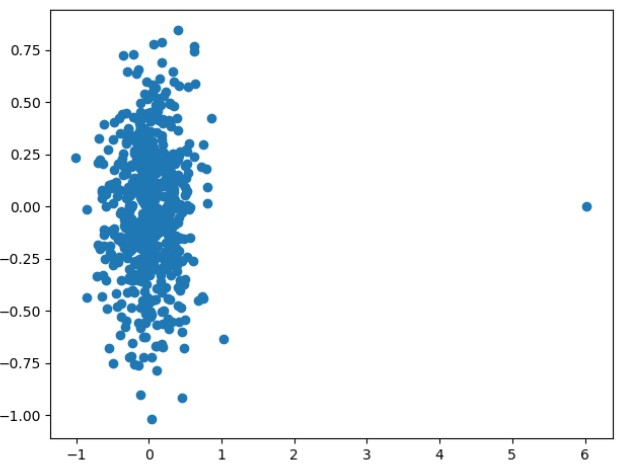
\includegraphics[width=.5\textwidth]{images/worst_blob_case.jpg}
        \caption{Output of the \texttt{worst\_blob\_case} function with \texttt{gen\_pam = 5.0}.}
        \label{fig:worst-blob-case}
    \end{figure*}
    
\begin{itemize}
    \item[1.2.] \textbf{What happens when you change the generating parameter of \texttt{worst\_case\_blob} in \linebreak
    \texttt{how\_to\_choose\_espilon} and run the function? What if the parameter is very large?}
\end{itemize}
    
    In the function \texttt{how\_to\_choose\_epsilon}, in order to ensure connectivity of the graph, the value of $\epsilon$ is chosen thanks to a minimum spanning tree (MST) over the dataset, \ie, we choose $\epsilon$ as the largest distance in the MST (or equivalently, the smallest similarity). The problem is that it is not robust to outliers. Indeed, a point too far from the other points will increase the longest distance in the MST, and thus the value of $\epsilon$. This makes the thresholding useless, and the graph fully-connected (or almost). In figure \ref{fig:gen-pam-influence}, we notice that the adjacency matrix is sparse when there is no outlier, \ie, when $\texttt{gen\_pam} = 0$. But when we increase the value to $1$, it is almost fully-connected, and when $\texttt{gen\_pam} = 2$, the graph is (except for the outlier) fully-connected.
    
    \begin{figure}[!ht]
     \begin{minipage}{0.48\textwidth}
     \begin{center}
         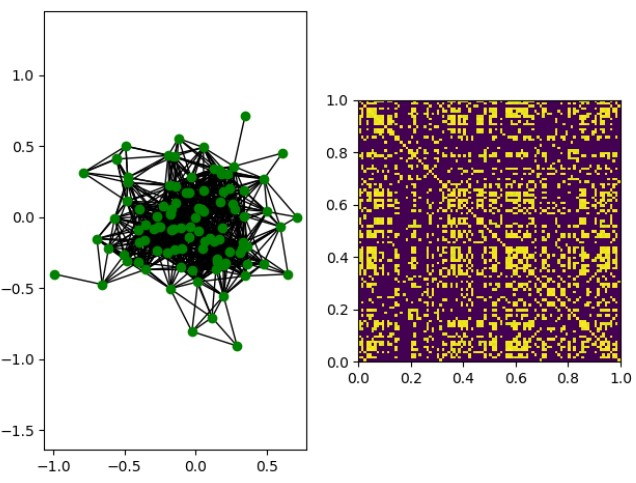
\includegraphics[width=\textwidth]{images/gen_pam_0.jpg}
         \caption{$\texttt{gen\_pam} = 0$}
     \end{center}
     \end{minipage}
     \hfill
     \begin{minipage}{0.48\textwidth}
     \begin{center}
         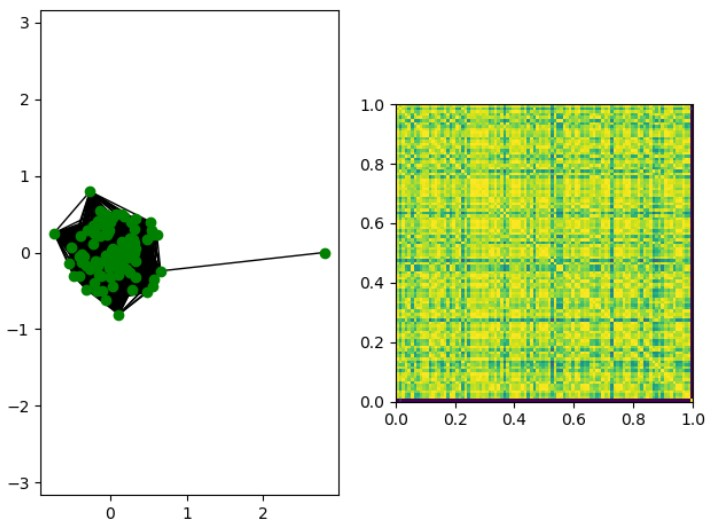
\includegraphics[width=\textwidth]{images/gen_pam_2.jpg}
         \caption{$\texttt{gen\_pam} = 2$}
     \end{center}
     \end{minipage}
        \caption{Evolution of the graph and the adjacency matrix when the value of \texttt{gen\_pam} increases. Although the adjacency matrix is sparse when $\texttt{gen\_pam} = 0$, it becomes dense when $\texttt{gen\_pam} = 2$.}
        \label{fig:gen-pam-influence}
    \end{figure}
    
    \pagebreak
    
\begin{itemize}
    \item[1.3.] \textbf{Using \texttt{plot\_similarity\_graph} and one of the datasets, compare k-nn to $\epsilon$ graphs. When is it easier to build a connected graph using k-nn? When using $\epsilon$ graphs?}
\end{itemize}

    Let's take the example of the blobs dataset. In figure \ref{fig:blobs-dataset}, we take $\epsilon = 0.5$ (on the left) and $k = 20$ (on the right). In this case, \ie, when the dataset contains compact regions (here, the three blobs) that are relatively far from each other, the k-nn graph breaks the dataset in three disconnected components. If we want to have a connected graph, we need a high value for $k$, (\eg higher than the number of points in each cluster).
    
    For the $\epsilon$ graph, as each cluster is very dense, each cluster is fully-connected (or almost), whereas different clusters are "almost not" connected. If we had different densities for each cluster, it would result in huge differences between the clusters, \ie, points inside a cluster could be tightly connected whereas points inside another cluster almost not connected. This can be solved by using the k-nn graph (not here, as explained just above).
    
    \begin{figure}[!ht]
     \begin{minipage}{0.48\textwidth}
     \begin{center}
         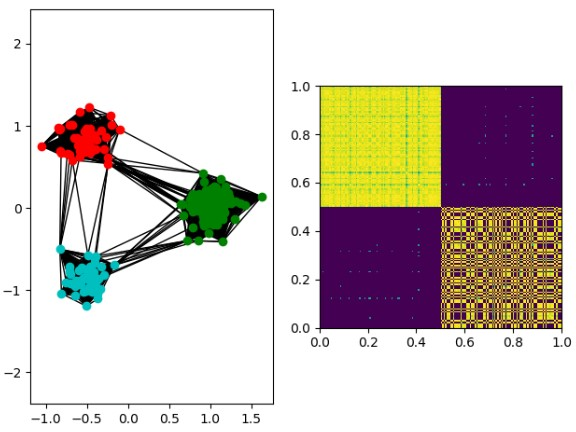
\includegraphics[width=\textwidth]{images/eps_05_blobs.jpg}
         \caption{$\epsilon = 0.5$}
     \end{center}
     \end{minipage}
     \hfill
     \begin{minipage}{0.48\textwidth}
     \begin{center}
         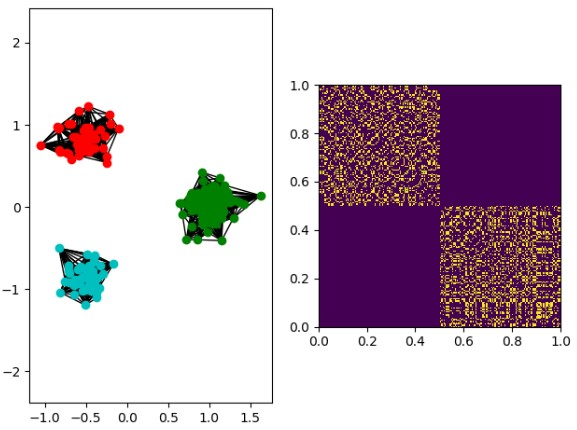
\includegraphics[width=\textwidth]{images/knn_20_blobs.jpg}
         \caption{$k = 20$}
     \end{center}
     \end{minipage}
        \caption{Comparison between $\epsilon$ graph and k-nn graph.}
        \label{fig:blobs-dataset}
    \end{figure}



\section{Spectral clustering}



\begin{itemize}
    \item[2.1.] \textbf{Build a graph starting from the data generated in \texttt{two\_blobs\_clustering}, and remember to keep the graph connected. Motivate your choice on which eigenvectors to use and how you computed the clustering assignments from the eigenvectors. Now compute a similar clustering using the built-in k-means and compare the results.}
\end{itemize}
    
    As the graph is connected, $0$ has a multiplicity of $1$ as an eigenvalue of the Laplacian matrix and a corresponding eigenvector is constant. Hence, it is not useful for the clustering. So one could take the following eigenvectors to make the clustering. In this case - as there are two clusters - we know by the Rayleigh-Ritz theorem that the second eigenvector, $f_{2}$, of the Laplacian matrix approximates a minimizer of RatioCut (or NCut, depending on which Laplacian is used). To compute the clustering assignments, it is possible to threshold $f_{2}$ at $0$ and choose to put the negative components' indices in a cluster, and the positive ones in the other. One could also apply the $k$-means algorithm on the components of the vector. More generally, for $k$ clusters, one could take the $k$ first eigenvectors (drop the first one is the graph is connected) to form a matrix $U \in \R^{n \times k}$ and apply $k$-means algorithm on U's rows. The choice of the eigenvectors is, once again, justified by a version of the Rayleigh-Ritz theorem. \\
    
    Now, let compute the two blobs clustering. As we want to have a connected graph, we use here a $\epsilon$-graph, computed using a minimum spanning tree. In figure \ref{fig:two-blobs-21-eigenvectors} are shown the first and second eigenvectors of the Laplacian. We see that the first eigenvector is constant, and thus not useful for the clustering. As mentioned above, we could use the sign of each component of the second eigenvector to compute the cluster assignments. In the code, we use the $k$-means algorithm in order to be a bit more general, but those two methods lead - in this case - to the same results.

    \begin{figure*}[!ht]
        \centering
        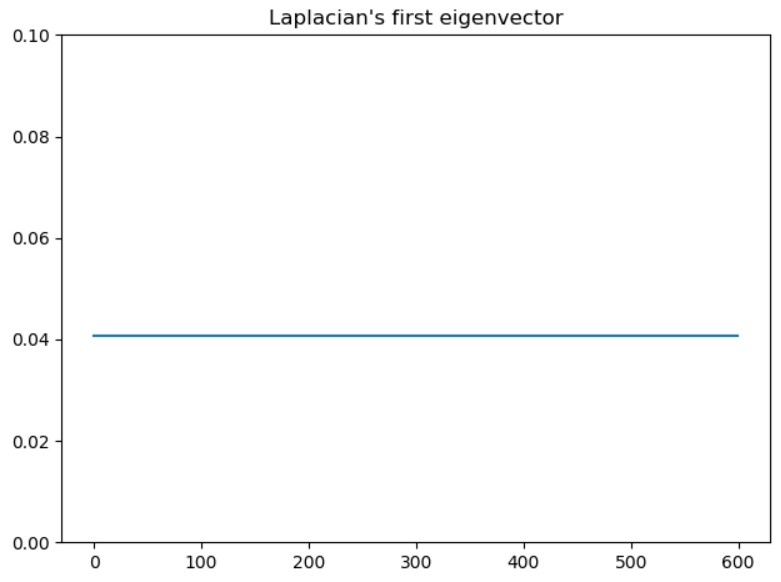
\includegraphics[width=.48\textwidth]{images/two_blobs_21_first_eigenvector.jpg}
        \hfill
        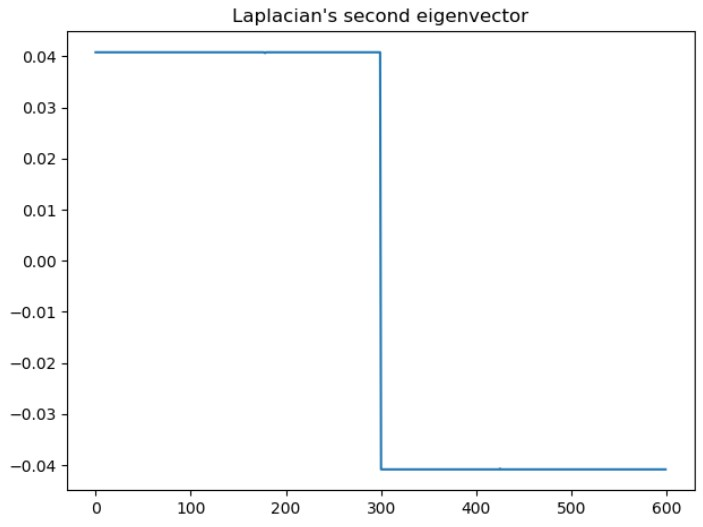
\includegraphics[width=.48\textwidth]{images/two_blobs_21_second_eigenvector.jpg}
        \caption{First and second eigenvectors of the Laplacian.}
        \label{fig:two-blobs-21-eigenvectors}
    \end{figure*}

    In figure \ref{fig:question-21-results}, there are the results of the clustering assignments obtained from spectral clustering and from a $k$-means on the original data set. There is also the ground-truth in order to compare with our results. We see that the three coincide.
    
    \begin{figure*}[!ht]
        \centering
        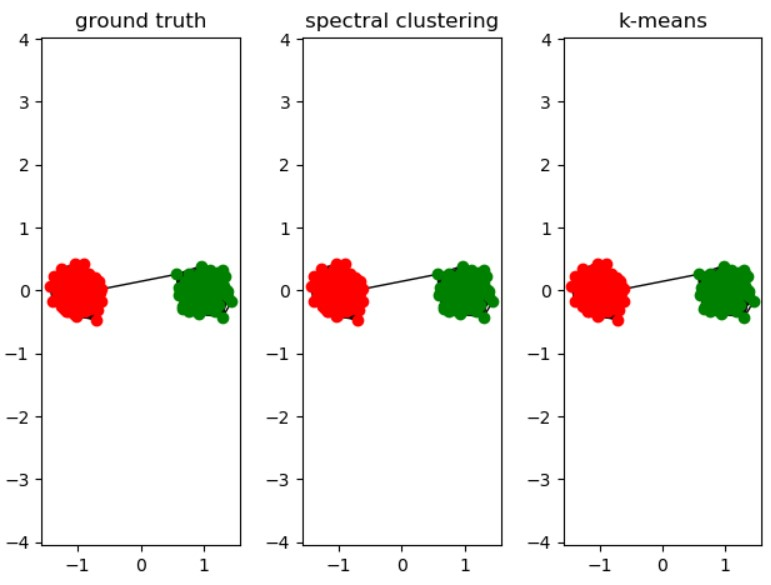
\includegraphics[width=.5\textwidth]{images/question_21_results.jpg}
        \caption{Results of spectral clustering and $k$-means on original data.}
        \label{fig:question-21-results}
    \end{figure*}
    
    \pagebreak
    
\begin{itemize}
    \item[2.2.] \textbf{Build a graph starting from the data generated in \texttt{two\_blobs\_clustering}, but this time make it so that the two components are separate. How do you choose which eigenvectors to use in this case? Motivate your answer.}
\end{itemize}

    Here, we compute the $k$-nn graph with $k = 20$. It has two separated components. Thus, the first eigenvector is not constant anymore (see figure \ref{fig:two-blobs-22-eigenvectors}), we can use it for computing the cluster assignments. We take the two first eigenvectors of the Laplacian, that - up to a constant - correspond to the indicator vectors of each cluster.
    
    \begin{figure*}[!ht]
        \centering
        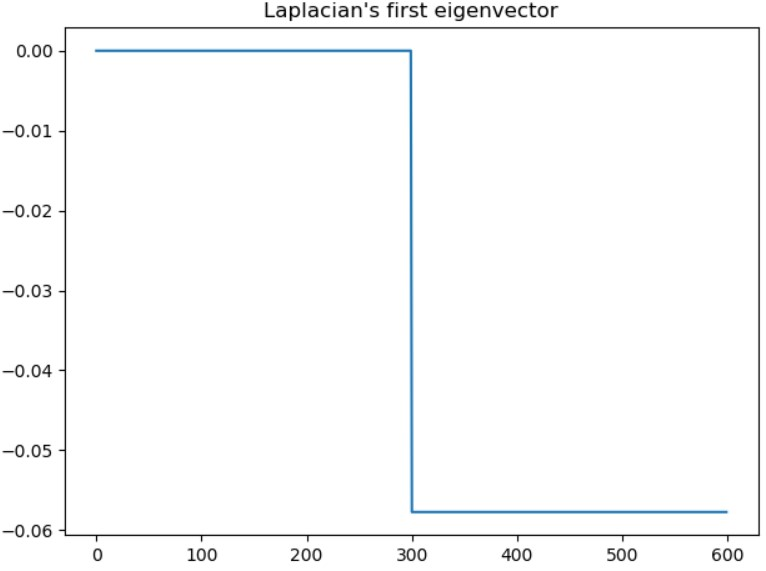
\includegraphics[width=0.48\textwidth]{images/two_blobs_22_first_eigenvector.jpg}
        \hfill
        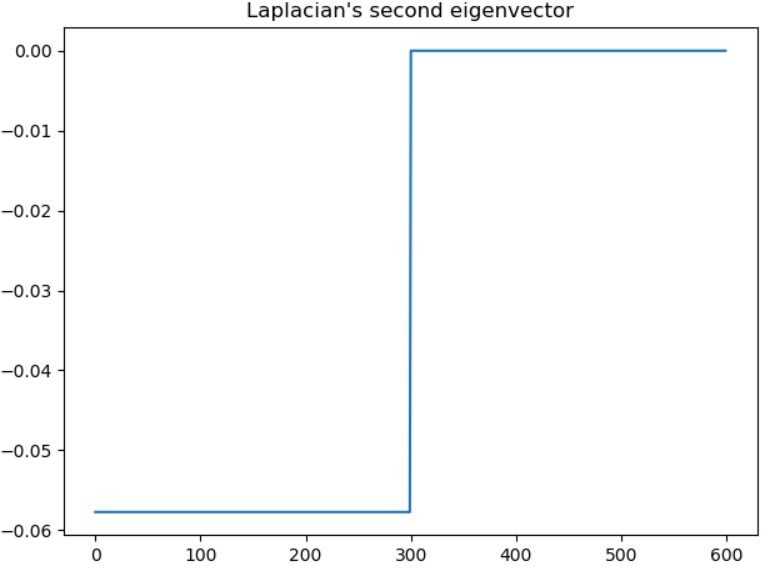
\includegraphics[width=0.48\textwidth]{images/two_blobs_22_second_eigenvector.jpg}
        \caption{First and second eigenvectors of the Laplacian.}
        \label{fig:two-blobs-22-eigenvectors}
    \end{figure*}

    The results are shown in figure \ref{fig:question-22-results}. As in question 2.1., the results coincide with the ground-truth.
    
    \begin{figure*}[!ht]
        \centering
        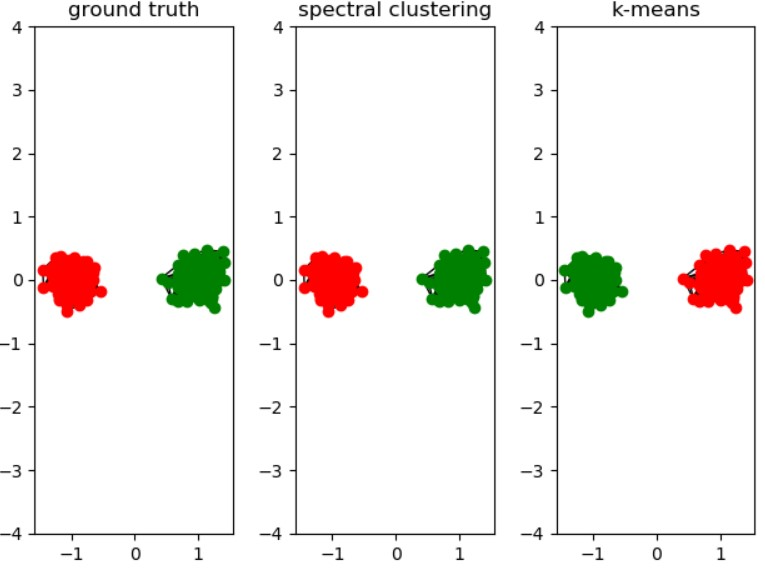
\includegraphics[width=.5\textwidth]{images/question_22_results.jpg}
        \caption{Results of spectral clustering and $k$-means on original data.}
        \label{fig:question-22-results}
    \end{figure*}

    \pagebreak

\begin{itemize}
    \item[2.3.] \textbf{Look at the function \texttt{find\_the\_bend}. Generate a dataset with $4$ blobs and $\sigma^{2} = 0.03$. Build a graph out of it and plot the first $15$ eigenvalues of the Laplacian. Complete the function \texttt{choose\_eig\_function} to automatically choose the number of eigenvectors to include. The decision rule must adapt to the actual eigenvalues of the problem.}
\end{itemize}

    As mentioned above, when it comes to find $k$ clusters, taking the $k$ first eigenvectors of the Laplacian for the spectral clustering is justified by a version of the Rayleigh-Ritz theorem, and this no matter what the normalization is (unnormalized, symmetric or random walk). But when the number of clusters $k$ is unknown, one has to choose when to stop. For this purpose, one may look at the eigengaps between the eigenvalues (denoted $\lambda_{1} \leq \dots \leq \lambda_{n}$) of the Laplacian. The idea is to stop when $\lambda_{1}, \dots, \lambda_{k}$ are relatively small and $\lambda_{k+1}$ relatively large. A first attempt would be to take the index of the largest eigengap starting from the first non-zero eigenvalue, \ie, $k = \arg \max_{i} \lambda_{i+1} - \lambda_{i}$ but as a large gap can appear lately in the spectrum of the Laplacian, it does not check if the eigenvalues before the gap are "relatively small" and the eigenvalue after the gap is "relatively large". Hence, to take the latter remark in account, one might take:
    
    \[ k = \arg \max_{i} \frac{\lambda_{i+1} - \lambda_{i}}{\sum_{j=1}^{i} \lambda_{j} + \epsilon} \]

    or simply

    \[ k = \arg \max_{i} \frac{\lambda_{i+1} - \lambda_{i}}{\lambda_{i+1} + \lambda_{i} + \epsilon} \]

    where $\epsilon$ is just a small number to avoid division by zero (fixed to $\epsilon = 10^{-9}$ in the code). In this particular case ($4$ blobs and small variance), the first heuristic takes the six first eigenvalues and does not cluster the data perfectly. The two latter take the four first eigenvalues and return a better clustering. See figure \ref{fig:find-the-bend}.

    \begin{figure*}[!ht]
        \centering
        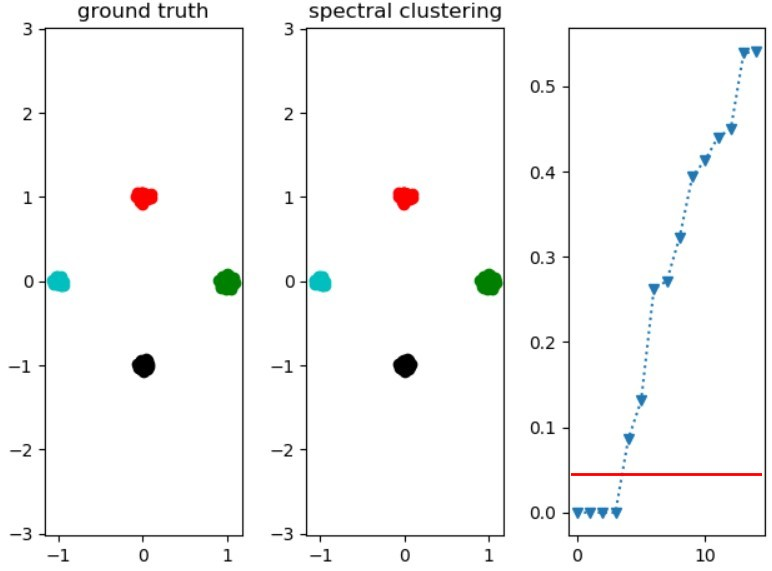
\includegraphics[width=.5\textwidth]{images/find_the_bend.jpg}
        \caption{Eigenvalues kept by the function \texttt{choose\_eigenvalues} are below the red line in the third panel.}
        \label{fig:find-the-bend}
    \end{figure*}

    \pagebreak

\begin{itemize}
    \item[2.4.] \textbf{Now increase the variance of the Blobs to $\sigma^{2} = 0.20$ as you keep plotting the eigenvalues. Use the function \texttt{choose\_eig\_function}. Do you see any difference?}
\end{itemize}

    When the variance increases, the blobs are less separated. Thus, it becomes harder to choose the right $k$. For some data sets, we may have a very smooth spectrum without "big" eigengap, making the choice of $k$ hard. In figure \ref{fig:question-24-results} (where the parameter for the $k$-nn graph is $10$), the right $k$ has been found but if we run several times the algorithm, it is not always the case.

    \begin{figure*}[!ht]
        \centering
        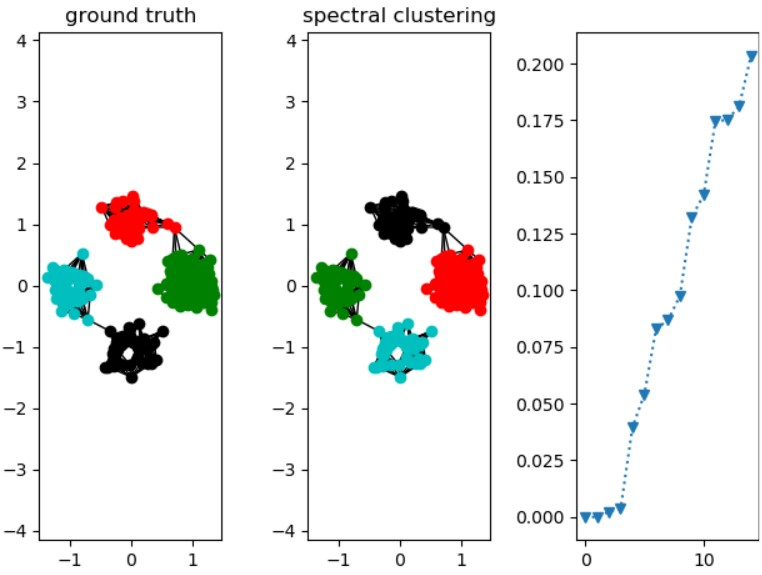
\includegraphics[width=.5\textwidth]{images/question_24_results.jpg}
        \caption{$4$ blobs with a variance of $0.2$.}
        \label{fig:question-24-results}
    \end{figure*}

\begin{itemize}
    \item[2.5.] \textbf{When you built the cluster assignment, did you use thresholding, $k$-means or both? Do you have any opinion on when to use each?}
\end{itemize}

    As mentionned in the question 2.1., both methods were tried but as the thresholding gave the same results than the $k$-means, it is the $k$-means method that is implemented in the code, in order to be more general. Indeed, the first one may be used when the data set is simple but in general, the heuristic might be too simple. Hence, we keep the $k$-means method.

\begin{itemize}
    \item[2.6.] \textbf{What is another use that looking at the distribution of the eigenvalues can have during clustering, besides choosing which eigenvectors to include?}
\end{itemize}

    The distribution of the eigenvalues can also give us the number of connected components in the graph, which is equal to the multiplicity of the eigenvalue $0$. We also know that the $k$-th eigenvalue is the smoothness of the $k$-th eigenvector.

\begin{itemize}
    \item[2.7.] \textbf{Plot your results using spectral clustering and $k$-means in \texttt{two\_moons\_clustering} and compare the results. Do you notice any difference? Taking into consideration the graph structure, can you explain them?}
\end{itemize}

    In figure \ref{fig:question-27-results}, we can see that the spectral clustering performs well, whereas the $k$-means algorithm fails. As $k$-means tries to find compact clusters, it cannot find clusters that are connected but not compact. But the Laplacian separates the different connected components, hence it makes such a clustering easy.

    \begin{figure*}[!ht]
        \centering
        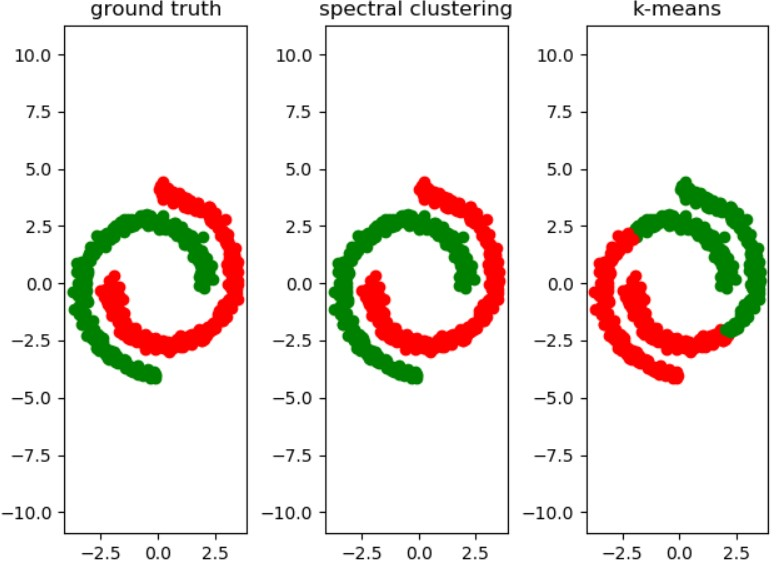
\includegraphics[width=.5\textwidth]{images/question_27_results.jpg}
        \caption{Two-moons data set clustering ($\epsilon = 0.8$).}
        \label{fig:question-27-results}
    \end{figure*}

\begin{itemize}
    \item[2.8.] \textbf{In the function \texttt{point\_and\_circle\_clustering}, compare spectral clustering using the normal laplacian $L$ and the random-walk regularized Laplacian $L_{rw}$. Do you notice any difference? Taking into consideration the graph structure, can you explain them?}
\end{itemize}

    \begin{figure*}[!ht]
        \centering
        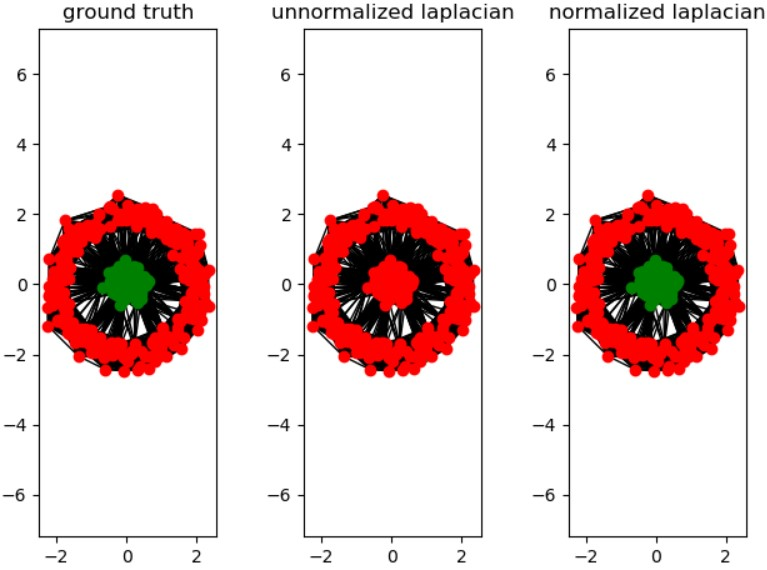
\includegraphics[width=.5\textwidth]{images/question_28_results.jpg}
        \caption{Point and circle data set clustering ($\epsilon = 0.4$).}
        \label{fig:question-28-results}
    \end{figure*}

    In figure \ref{fig:question-28-results} we see that the normal Laplacian fails to find the clusters whereas the normalized Laplacian finds them. We can try to explain it using the link to RatioCut and NCut minimization problems. We know that using the normal Laplacian can help minimizing RatioCut, whereas the normalized Laplacian can minimize NCut. If both methods minimize the cut between the two clusters (\ie minimize the between-cluster similarity), they behave differently when it comes to the within-cluster similarity, which is to be maximized. Indeed, in RatioCut, we want to maximize the number of vertices in the clusters. This number is not necessarily related to the within-cluster similarity. But for NCut, we want to maximize the volume of the clusters, which depends on the weights of the edges. Hence it is related to the within-cluster similarity. That is why, in this case, the normalized Laplacian can separate the point and the circle and the unnormalized cannot.

\begin{itemize}
    \item[2.9.] \textbf{Complete the function \texttt{parameter\_sensitivity}, and generate a plot of the ARI index while varying one of the parameters in the graph construction $\epsilon$ or $k$. Comment on the stability of the spectral clustering.}
\end{itemize}

    We generate the two moons data set with $500$ samples, we take the random walk normalization for the Laplacian and we use the adaptative spectral clustering to compute the clustering assignments. In figure \ref{fig:ari-eps} and \ref{fig:ari-knn}, we show the evolution of the ARI as a function of the $\epsilon$ parameter or the $k$ parameter. We see that the choice of the parameter is very important in the sense that, depending on its value, the score can be very low or very high. Besides, it seems that the graphs are a bit smooth, \ie there is not a single appropriated value but a wide range of it, \eg in order to have a high score, we can take $\epsilon \in [0.7, 0.9]$ or $k \in [\![ 5, 20 ]\!]$. In brief, the choice of the similarity graph is very important.

    \begin{figure*}[!ht]
    \begin{minipage}{.45\textwidth}
        \centering
        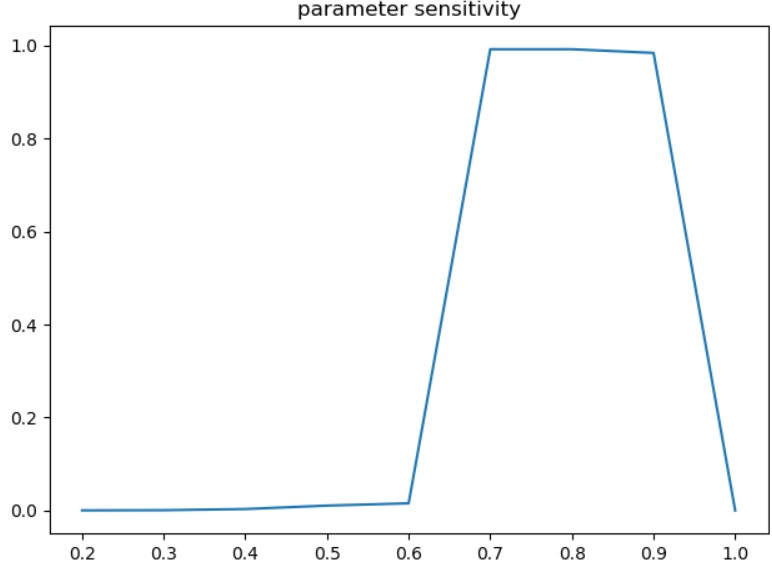
\includegraphics[width=\textwidth]{images/ari_eps.jpg}
        \caption{Sensitivity to $\epsilon$ when building the $\epsilon$ graph. The plot represents the ARI as a function of $\epsilon$.}
        \label{fig:ari-eps}
    \end{minipage}
    \hfill
    \begin{minipage}{.45\textwidth}
        \centering
        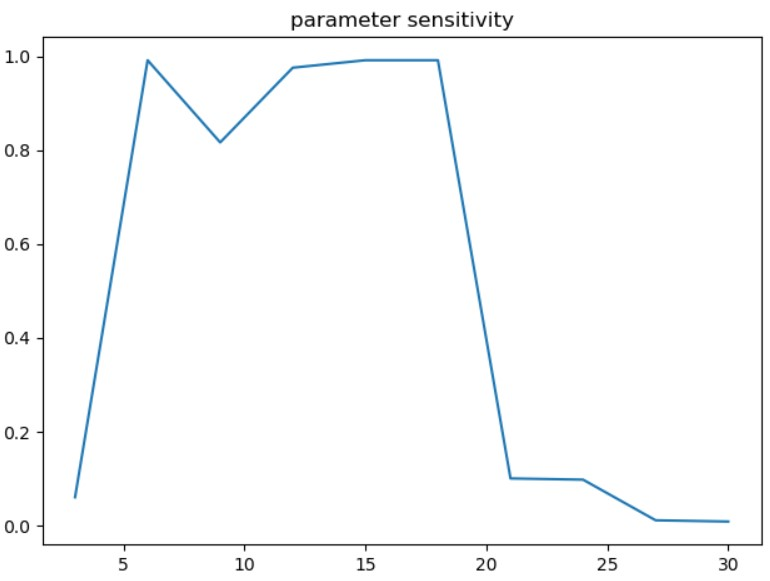
\includegraphics[width=\textwidth]{images/ari_knn.jpg}
        \caption{Sensitivity to $k$ when building the $k$-nn graph. The plot represents the ARI as a function of $k$.}
        \label{fig:ari-knn}
    \end{minipage}
    \end{figure*}

\begin{itemize}
    \item[2.10.] \textbf{If we did not have access to \textit{true} labels how could we evaluate the clustering result (or what should we not use as evaluation)?}
\end{itemize}

    An usual metric to assess the quality of a clustering $C : V \longrightarrow \lbrace 1, \dots, K \rbrace$ is the modularity, defined by:

    \[ Q(C) = \frac{1}{2w} \sum_{i, j \in V} \left( A_{ij} - \frac{w_{i}w_{j}}{2w} \right) \delta_{C(i), C(j)} \]

    \noindent where $A$ is the adjacency matrix, $w_{i} = \sum_{j \in V} A_{ij}$ and $w$ the total weight of edges.

    Let define the \emph{strength} of a cluster $k$ as the quantity: $\rho_{k} = \frac{2 w_{k}}{v_{k}}$ where $v_{k} = \sum_{i: C(i) = k} d_{i}$ is the volume of the cluster $k$. Interpreting modularity through random walks, it is possible to show that $\rho_{k}$ is the probability that given that the random walk is in cluster $k$, it stays in cluster $k$ after one move. Denoting $\pi_{k}$ the probability that the random walk lies in cluster $k$, the modularity can be expressed as:

    \[ Q(C) = \sum_{k=1}^{K} \pi_{k} \left( \rho_{k} - \pi_{k} \right) \]

    Modularity is the quantity that is to be maximized in the Louvain algorithm. In general, one should be looking for a metric that relies both on between-cluster similarity and within-cluster similarity, and not only on the between-cluster similarity.

\section{Image Segmentation}

    Here are the results obtained for the segmentation:

    \begin{figure*}[!ht]
        \centering
        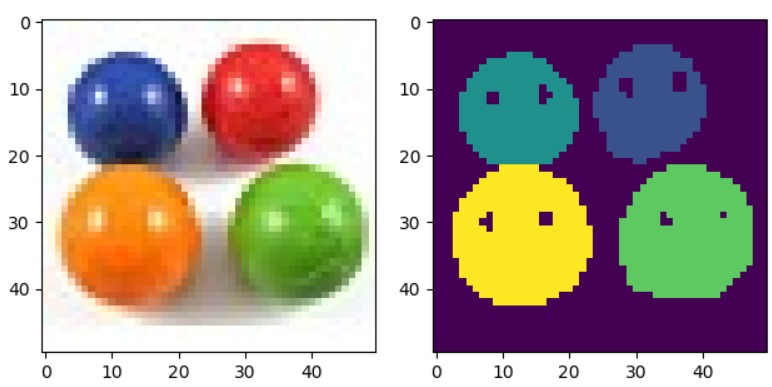
\includegraphics[scale=0.65]{images/four_elements_segmentation.jpg}
        \caption{Segmentation in five classes ($k$-nn graph).}
        \label{fig:four-elements-segmentation}
    \end{figure*}

    \begin{figure*}[!ht]
        \centering
        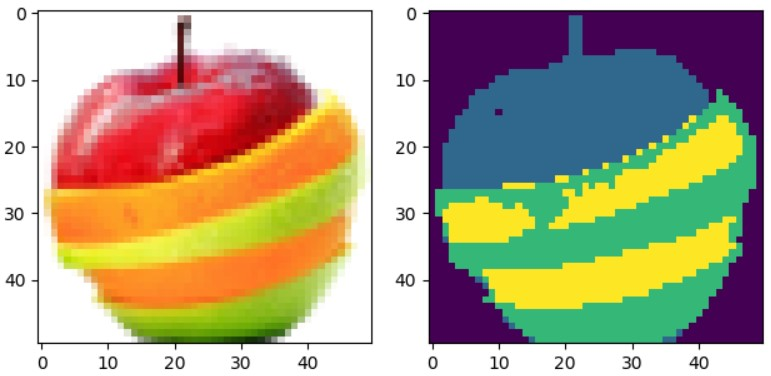
\includegraphics[scale=0.65]{images/fruit_salad_segmentation.jpg}
        \caption{Segmentation in four classes ($k$-nn graph).}
        \label{fig:fruit-salad-segmentation}
    \end{figure*}


\begin{itemize}
    \item[3.1.] \textbf{The first documentation is the code. If your code is well written and well commented, that is enough. If you think you need to better express some choices you made in the implementation, you can use this question in the report. Remember to include all the related code in the submission.}
\end{itemize}
    
    Nothing to say.
    
\begin{itemize}
    \item[3.2.] \textbf{A full graph built between the pixels of a $50 \times 50$ image corresponds to $50^{2}$ nodes. Solving the full eigenvalue problem in this case would scale in the order of $2^{34}$. Even on weak hardware (\ie iPhone) this takes only seconds to minutes. Segmenting a Full HD picture of $1920 \times 1080$ would scale in the order of $2^{64}$ (about a month on a decent machine \ie not an iPhone). Beyond that, the large picture would require to store in memory a graph over millions of nodes. A full graph on that scale requires about $1 TB$ of memory. Can you think two simple techniques to reduce the computational and occupational cost of Spectral Clustering?}
\end{itemize}
    
    A first idea would be to apply spectral clustering on a downsampled version of the image in order to reduce the number of nodes in the graph and then to upsample the segmentation obtained in order to fit to the original image.
    
    Another idea would be to generate super-pixels using methods such as SLIC and to create the graph from these super-pixels. In figure \ref{fig:super-pixels} is shown an example of super-pixels.
    
    \begin{figure*}[!ht]
        \centering
        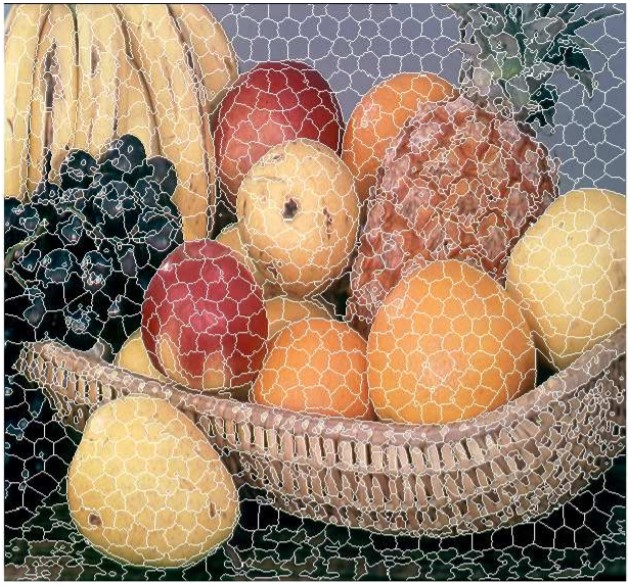
\includegraphics[scale=0.65]{images/super_pixels.jpg}
        \caption{Example of super-pixels.}
        \label{fig:super-pixels}
    \end{figure*}
    
    Besides, using $k$-nn graph instead of $\epsilon$ graph may speed up the algorithm as it usually results in more sparse matrices.

\begin{itemize}
    \item[3.3.] \textbf{Did you use \texttt{eig} or \texttt{eigs} to extract the final eigenvectors? Shortly, what is the difference between the two? How do they scale to large graphs (order of complexity)?}
\end{itemize}
    
    In the attached code, it is the function \texttt{scipy.linalg.eig} which is used. The main difference between those two functions is that \texttt{scipy.sparse.linalg.eigs} uses the "Implicitly Restarted Arnoldi Methods" and probably takes better advantage of the sparsity of the matrix. Besides, as the Laplacian is symmetric, one could have used \texttt{scipy.linalg.eigh} or \texttt{scipy.sparse.linalg.eigsh}.

\end{document}